\documentclass[varwidth,margin=1in]{standalone}

\usepackage{amsmath}
\usepackage[margin=1in]{geometry}
\usepackage[russian]{babel}
\usepackage{amssymb}
\usepackage{derivative}
\usepackage[utf8]{inputenc}
\usepackage{graphicx}

\title{Контрольная работа\\ по решению уравнений и систем уравнений\\
% Вопрос 1
Вопрос 1 and 2
}
\date{}

\begin{document}

\maketitle

\begin{figure}[h!]
    \centering
    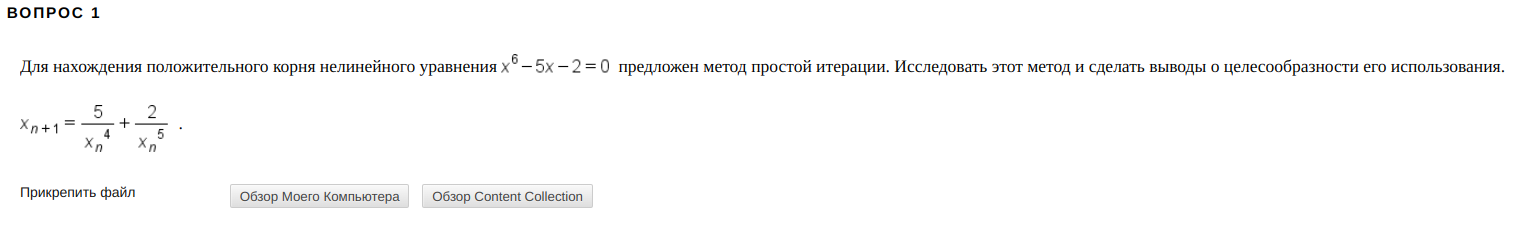
\includegraphics[width=\linewidth]{q1.100,00
    100,00
    }
\end{figure}

Предлагаемая формула для использования в методе простой итерации была следующей:


\[x^6-5x-2 =0\]
\[x^6      =5x+2\]
\[x        =\frac{5}{x^4}+\frac{2}{x^5}\]

\[\therefore x_{n+1} = \frac{5}{x_n^4}+\frac{2}{x_n^5}\]

Чтобы проверить, работает ли эта функция для метода простой итерации (т. е. сходится ли она), мы должны проверить следующее:

\[\left|\odv{}{x}\left(\frac{5}{x^4}+\frac{2}{x^5}\right)\right|<1, \: \forall x \in I, \: x_{\text{корень}} \in I\]

Сверяясь с Desmos, получаем следующий график:

\begin{figure}[h!]
    \centering
    \includegraphics*[width=\linewidth]{deriv.png}
\end{figure}

Там мы видим, что при значениях \(x\) меньше 2 наш метод будет расходиться. Поэтому нам нужно проверить, есть ли корни в этом интервале \((0,2)\).

\begin{figure}[h!]
    \centering
    \includegraphics*[width=0.75\linewidth]{fun.png}
\end{figure}

Как видно, единственный положительный корень (поскольку при всех \(x>2\) все значения производных функции положительны) находится в этом интервале, где модуль нашей производной больше 1. Это означает, что эта функция не привести к корню и метод будет расходиться.

\begin{figure}[h!]
    \centering
    \includegraphics*[width=\linewidth]{q2.png}
\end{figure}

\[F(u)=
    \left(
    \begin{matrix}
            x-y^3-1 \\
            (x+3)(y-1)-5
        \end{matrix}
    \right)
\]

\[J=
    \left(
    \begin{matrix}
            1   & -3y^2 \\
            y-1 & x+3
        \end{matrix}
    \right)
\]

\[J^{-1}=
    \frac{1}{x+3-(-3y^2)(y-1)}
    \left(
    \begin{matrix}
            x+3 & 3y^2 \\
            1-y & 1
        \end{matrix}
    \right)
\]

Используя \(M=(0,0)\) в качестве начального приближения:

\[
    u_{1} =
    \left(
    \begin{matrix}
            0 \\
            0
        \end{matrix}
    \right)
    +
    \frac{1}{0+3-(-3 \cdot 0^2)(0-1)}
    \left(
    \begin{matrix}
            0+3 & 3 \cdot 0^2 \\
            1-0 & 1
        \end{matrix}
    \right)
    \cdot
    \left(
    \begin{matrix}
            0-0^3-1 \\
            (0+3)(0-1)-5
        \end{matrix}
    \right)
\]
\[
    u_{1} =
    \left(
    \begin{matrix}
            0 \\
            0
        \end{matrix}
    \right)
    +
    \frac{1}{3}
    \left(
    \begin{matrix}
            3 & 0 \\
            1 & 1
        \end{matrix}
    \right)
    \cdot
    \left(
    \begin{matrix}
            -1 \\
            -8
        \end{matrix}
    \right)
    =
    \left(
    \begin{matrix}
            -1 \\
            -3
        \end{matrix}
    \right)
\]
\[
    \vdots
\]

Используя больше итераций, мы видим, что использование \(M=(0,0)\) в качестве начального приближения расходится.

\[ u_{0} = \left(\begin{matrix} 0 \\ 0 \end{matrix}\right) \]
\[ u_{1} = \left(\begin{matrix} -1.0 \\ -3.0 \end{matrix}\right) \]
\[ u_{2} = \left(\begin{matrix} 1.8396226415094339 \\ -3.8207547169811322 \end{matrix}\right) \]
\[ u_{3} = \left(\begin{matrix} 6.526038850197102 \\ -5.006502255327961 \end{matrix}\right) \]
\[ u_{4} = \left(\begin{matrix} 14.284907091290336 \\ -6.645642562719063 \end{matrix}\right) \]
\[\vdots\]
\[ u_{97} = \left(\begin{matrix} 8.542782266737642e+21 \\ -2791904605926.876 \end{matrix}\right) \]
\[ u_{98} = \left(\begin{matrix} 1.4237970444563757e+22 \\ -3722539474569.168 \end{matrix}\right) \]
\[ u_{99} = \left(\begin{matrix} 2.372995074094087e+22 \\ -4963385966092.225 \end{matrix}\right) \]

\end{document}